\chapter{Introduction}

Economics has been defined as the study of making the best use of scarce resources, that is, of maximization subject to constraints. The criterion being maximized, and the constraints imposed on the choice, vary from one context to the next: households' consumption and labor supply, firms' production, and governments' policies. But all constrained maximization problem have a common economic intuition for them. This book aims to outline the mathematics and develop the intuition.

The standard model of a consumer's choice provides a good point of departure. The basic concepts are a budget line and a set of indifference curves. The points on the budget line represent all affordable combinations of two goods. The family of indifference curves represents the objective, namely to reach as high a curve as possible. The optimum is where an indifference curve is tangential to the budget line. Figure \ref{Fig1.1} shows the familiar picture.

In this chapter I shall develop this model further, using verbal and geometric arguments, but with an eye toward the mathematical sharpening and generalization that will occupy us in later chapters.

It helps to give a little algebraic content to the various magnitudes in Figure \ref{Fig1.1}. Write $I$ for the consumer's money income, $p_1$ and $p_2$ for the prices of the two goods, and $x_1$ and $x_2$ for their quantities. The budget line, where the expenditure exactly equals income, can then be expressed by the equation

%\begin{figure}[!htb] %H为当前位置,!htb为忽略美学标准,htbp为浮动图形
%\centering %图片居中
%\includegraphics[width=0.8\textwidth]{./Fig1.1.png} %插入图片,[]中设置图片大小,{}中是图片文件名
%\caption{The consumer's optimum choice} %最终文档中希望显示的图片标题
%\label{Fig1.1} %用于文内引用的标签
%\end{figure}


\begin{figure}[!tb] %H为当前位置,!htb为忽略美学标准,htbp为浮动图形
\centering %图片居中
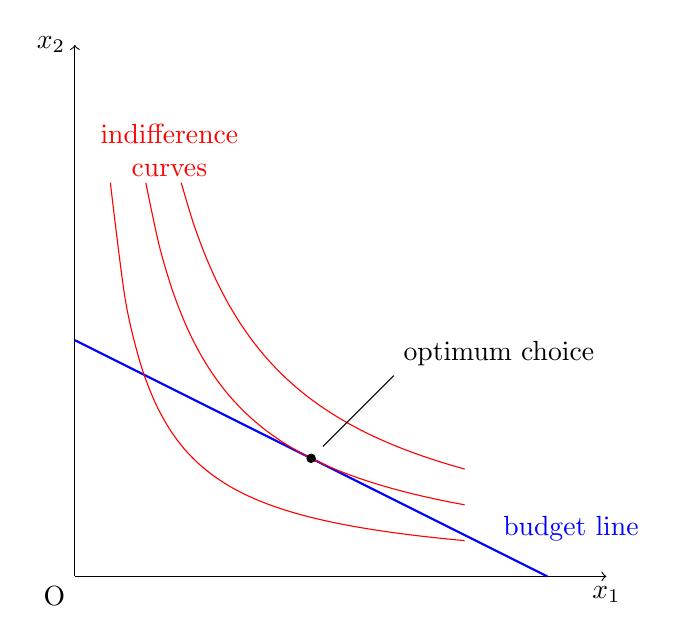
\begin{tikzpicture}[scale=1.5]
    % 绘制坐标轴
    \draw[->] (0,0) -- (4.5,0) node[below] {$x_1$};
    \draw[->] (0,0) -- (0,4.5) node[left] {$x_2$};
    \draw[black] (0,0) node[below left] {O};

% 预算约束线 x1 + 2 x2 = 4
    \draw[thick,blue] (0,2) -- (4,0) ; 
    \draw[thick,blue] (4.2,0.6) node[below] {budget line};

% 无差异曲线 x1 * x2 分别等于1,2,3
    \draw[domain=0.3:3.3,smooth,variable=\x,red] plot ({\x},{1/\x}) ;
    \draw[domain=0.6:3.3,smooth,variable=\x,red] plot ({\x},{2/\x}) ;
    \draw[domain=0.9:3.3,smooth,variable=\x,red] plot ({\x},{3/\x}) ;
    \draw[red] (0.8, 3.3) node[above, align=center] {indifference \\ curves};

% 标记均衡点(假设)
    \filldraw [black] (2,1) circle (1pt) ;
    \draw[black] (2.1, 1.1) -- (2.7,1.7) node[above right] {optimum  choice} ;
\end{tikzpicture}
\caption{The consumer's optimum choice} %最终文档中希望显示的图片标题
\label{Fig1.1} %用于文内引用的标签
\end{figure}


\begin{equation}\label{equa1.1}
p_1 x_1 + p_2 x_2 = I
\end{equation} 

The consumer's preferences over the amounts $x_1$ and $x_2$ of these goods are represented by a numerical scale, called the utility function. This assigns to each bundle $(x_1, x_2)$
of goods a number $U(x_1, x_2)$, called its utility level. In any comparison among alternative bundles, the preferred bundle is the one that receives the highest utility number. Along an indifference curve, all points must have the same utility number. Therefore such a curve has an equation

\begin{equation}\label{equa1.2}
U(x_1, x_2) = \mbox{constant}
\end{equation} 

The exposition of the theory now proceeds by calculating the slopes of the budget line and the indifference curve. For tangency between the two, the slopes must be equal. I shall do this soon. But let me begin with a much simpler and more intuitive approach.

\section*{The Arbitrage Argument}

The idea is to have the consumer start with any trial allocation of his budget, and contemplate a change. If this leads to a bundle of goods that he rates higher on his utility scale, then it is to be adopted as a new trial allocation. Once a bundle is found that cannot be bettered in this way, it will be the optimum allocation, and will be the one actually consumed. Thus the impossibility of finding an improvement will serve as the test of optimality.

The change does not entail any additional expenditures; it is merely a reallocation of some amounts of money from the purchaser of one good to the other. If the initial allocation is not optimal, this can raise the consumer's utility. When the consumer has made the best choice and reached his personal equilibrium, such opportunities for doing better with no net increase in expenditure vanish. This has a close parallel in financial markets. Outside a market equilibrium, participants can make `arbitrage' profits at a zero net outlay, taking advantage of discrepancies in prices of the same asset in different markets. In equilibrium there are no such opportunities. In fact, the very process of people seeking arbitrage profits brings about the equilibrium. I shall exploit this intuitive parallel by labeling this whole line of reasoning the `arbitrage argument', and the resulting optimality condition the `no-arbitrage argument'.

If goods are indivisible, these changes must occur in discrete steps. However, it is often a good approximation to suppose that goods are perfectly divisible. Then the changes can occur in infinitesimal amounts, or what economists call marginal adjustments. Even for seemingly indivisible goods, such as cars or other large consumer durables, there are dimensions of quality etc. that allow continuous adjustment. In any event, such marginal changes are the subject of our analysis in this book.

The standard symbol for `a small (marginal, infinitesimal) change in the variable $x$' is $dx$. This is not to be thought of as the product of two variables $d$ and $x$, but an entity $dx$ in its own right. The use of such infinitesimal magnitudes can be justified rigorously, but for the most part I shall use them in a loose heuristic way. Where you doubt a statement involving infinitesimals, or are unsure I have used them correctly, you should rework the argument using proper calculus methods, starting with a finite change $\Delta x$ and then going to the limit as $\Delta x \rightarrow 0$.

First suppose that initial allocation of the budget has positive amounts $x_1$ and $x_2$ of both goods. Now contemplate a small arbitrage operation, or a marginal reallocation of a small but positive amount of income $dI$ from good 2 to good 1. In physical terms, this means buying $dI/p_1$ units more of good 1 and $dI/p_2$ units less of good 2. Let $MU_1$ and $MU_2$ denote the marginal utilities of the two goods. This means that a small change $dx_1$ in the quantity of good 1 changes utility by $MU_1 dx_1$ units, and similarly $MU_2 dx_2$ for good 2. When the quantities of both goods are changing, the two effects can be added together, so the change in utility is

\begin{equation}\label{equa1.3}
MU_1 dx_1 + MU_2 dx_2
\end{equation} 

In later chapters I shall express this more rigorously using partial derivatives and Taylor series, but the simple statement will suffice here. The important point is that any one marginal adjustment is so small that any changes in the marginal utilities themselves during its course can be neglected. Of course if many such marginal adjustments are strung together, the marginal utilities will change gradually over this sequence. In particular, if $x_2$ rises and/or $x_1$ falls, $MU_2/MU_1$ will fall; this is the principle of the diminishing marginal rate of substitution in consumption. But for the moment I am speaking of just one marginal adjustment. 

The effect of the arbitrage operation on utility is then easy to compute. The increase of $dI/p_1$ in the quantity of good 1 raises utility by $MU_1 dI/p_1$, while the decrease of $dI/p_2$ in the quantity of good 2 lowers utility by $MU_2 dI/p_2$. The net increase in utility is therefore

\begin{equation*}
(MU_1 /p_1 - MU_2 /p_2) dI
\end{equation*} 

If this expression is positive, the consumer will carry out this reallocation and try further reallocation in the same direction. If the initial consumption bundle is optimum, therefore, the expression cannot be positive. This is a part of the `no-arbitrage' criterion of optimality. Since $dI$ was chosen positive, we can divide by it and write the criterion as 

\begin{equation}\label{equa1.4}
(MU_1 /p_1 - MU_2 /p_2) \leq 0
\end{equation} 

Now suppose the criterion is not met, that is, suppose the left-hand side expression in (\ref{equa1.4}) is > 0. Therefore some switch of expenditure toward good 1 is desirable. How far should this process go? Recall that as $x_1$ increases and $x_2$ decreases, $MU_1$ will gradually fall relative to $MU_2$. Eventually a point will be reached where the expression in (\ref{equa1.4}) is zero, and no further move in this direction can raise the consumer's utility level.

Next consider a reallocation in the opposite direction. This will switch the signs in all the above arguments. If the initial allocation is optimum, we must have

\begin{equation}\label{equa1.5}
(MU_1 /p_1 - MU_2 /p_2) \geq 0
\end{equation} 

If this if false, that is, if the expression is < 0, then the process of increasing $x_2$ and decreasing $x_1$ will be carried out until the expression reaches zero.

We can combine the two criteria of optimality of the initial consumption bundle into one: if the allocation $(x_1, x_2)$, with both quantities positive, is optimum, then the marginal utilities at this point must satisfy

\begin{equation}\label{equa1.6}
MU_1 /p_1 = MU_2 /p_2
\end{equation} 

This is the overall `no-arbitrage' condition. The economic interpretation is that at the optimum the consumer should be indifferent between allocating the marginal unit of money to the one good or the other.

\section*{The Tangency Condition Using Calculus}

The more complex but more commonly used way to derive the same condition of optimality is based on the tangency of the budget line (\ref{equa1.1}) and the indifference curve (\ref{equa1.2}). Write the equation of the budget line as 

\begin{equation*}
x_2 = (I/p_2) - x_1 (p_1 / p_2)
\end{equation*} 

Then we see at once that the slope of the line is $(p_1 / p_2)$ in numerical value. The slope of the indifference curve is the marginal rate of substitution(MRS) in consumption, and it equals the ratio of the marginal utilities $(MU_1 / MU_2)$. A heuristic derivation of this is as follows. If a marginal loss of $dx_1$ units of good 1 is just compensated by the marginal gains of $dx_2$ units of good 2, then the marginal rate of substitution(MRS) is the ratio $dx_2 / dx_1$. But the exact offset of the gain can be written as an equation in utility units

\begin{equation*}
MU_1 dx_1 = MU_2 dx_2
\end{equation*} 

Therefore

\begin{equation}\label{equa1.7}
MRS = dx_2 / dx_1 = MU_1 / MU_2
\end{equation} 

Incidentally, note the reversal of the subscripts 1 and 2 between the numerator and the denominator of the two ratios. This is not a typographical error; that is how the ratios are related, as you can see by cross-multiplying to get back to the equation just above.

At the optimum, the slope of the indifference curve (the marginal rate of substitution in consumption) is equal to the slope of the budget line (the price ratio). Therefore

\begin{equation}\label{equa1.8}
MU_1 / MU_2 = p_1 / p_2
\end{equation} 

This is equivalent to the optimality criterion (\ref{equa1.6}) we derived before. However, the verbal argument underlying (\ref{equa1.6}) has some advantages over the geometry of (\ref{equa1.8}). 

\section*{Corner Solutions}

The arbitrage argument is somewhat easier to adapt to the case where one of the goods is not bought at all. Since this occurs at one end or the other of the budget line, such optima are often called corner solutions. Suppose all income is spent on good 2 in the initial allocation, so $x_1 = 0$ and $x_2 = I/p_2$. Now of the two directions of improvement, namely trying to increase $x_1$ and to decrease it, only the former is possible. Therefore only the criterion (\ref{equa1.4}) corresponding to this test survives. Since $x_1$ cannot be decreased any further, the argument leading to (\ref{equa1.5}) cannot be made. The economic interpretation of (\ref{equa1.4}) holding for the consumption bundle $(0, I/p_2)$ is equally simple: even the first little units of income spent on good 1 does not bring enough utility benefit to match that from the last unit spent on good 2.

\section*{Marginal Utility of Income}

The second advantage of the arbitrage argument is even more important. Return to the situation where both goods are initially bought, and the criterion (\ref{equa1.6}) for optimality. Now suppose our consumer is given an extra amount $dI$ of income to spend. He could spend it all on good 1, buy $(dI/ p_1)$ more units of it and achieve an additional $(MU_1 dI/p_1)$ units of utility. Or he could spend it all on good 2, when his utility would increase by $(MU_2 dI / p_2)$ units. But the two increments to utility are equal by (\ref{equa1.6}). Therefore at the margin the allocation of the inifinitesimal amount $dI$ of extra income to good 1, or good 2, or indeed any mixture of the two, is a matter of indifference to the consumer. Then we can call the utility increment per unit of marginal addition to income simply the marginal utility of income, without bothering to specify how the marginal addition to the income is spent. Write $\lambda$ for this marginal utility of income. Then the $dI$ units of extra income raise utility by $\lambda dI$ units. Equating this to the two other ways of writing the same utility gain in terms of spending on each of the two goods, we find

\begin{equation}\label{equa1.9}
\lambda = MU_1 / p_1 = MU_2 / p_2
\end{equation} 

We see that the common value of the two sides in the optimality criterion (\ref{equa1.6}) has a very useful economic interpretation -- it is the marginal utility of income. A very similar interpretation is possible for the no-arbitrage conditions in all constrained optimization problems; I shall explain this in greater detail and unify it under the concept of Lagrange multipliers or shadow prices.

\section*{Many Goods and Constraints}

The generalization of the analysis to cover cases where there are several goods, some of which may not be bought at all, is equally easy. Suppose there are $n$ goods, with prices $(p_1, p_2, \dots, p_n$ and quantities $(x_1, x_2, \dots, x_n)$. For all goods bought in positive amounts at the optimum, the ratio of marginal utility to price must have a common value, which can then be interpreted as the marginal utility of income $\lambda$. For all goods not bought, the ratio of marginal utility to price must be smaller than, or at best equals to, this value. In symbols, for any goods $i$,

\begin{equation*}
MU_i / p_i \left\{  \begin{array}{lll}
=\lambda & \mbox{if} & x_i > 0 \\
\leq \lambda & \mbox{if} & x_i=0
\end{array}
\right.
\end{equation*} 

or

\begin{equation} \label{equa1.10}
MU_i - \lambda p_i \left\{  \begin{array}{lll}
=0 & \mbox{if} & x_i > 0 \\
\leq 0 & \mbox{if} & x_i=0
\end{array}
\right.
\end{equation} 

The method can also be extended to allow several constraints. We need a separate $\lambda$ for each constraints, and it can be interpreted as the marginal utility of relaxing that constraint. I shall discuss this in Chapter 3.

\section*{Non-binding Constraints}

Finally, consider an extension that is not of great relevance in consumer theory, but will prove very important in some other applications. Picture a consumer with an income so large that he is satiated, and fails to spend it all. The budget equation (\ref{equa1.1}) should be replaced by an inequality

\begin{equation*}
p_1 x_1 + p_2 x_2 \leq I
\end{equation*} 

We can bring this within the scope of the above theory simply by defining a new good $x_3$, `unspent income', which has price equal to one and yield no utility. (Note that I am not talking of saving, which enables a non-satiated consumer to spend more on desired goods in the future, but of totally useless unspent income.) The budget equation becomes

\begin{equation*}
p_1 x_1 + p_2 x_2 + x_3 = I
\end{equation*} 
and we have $MU_3 \equiv 0$. Since we are supposing that the consumer is choosing a positive amount of $x_3$, (\ref{equa1.10}) for $i=3$ gives $\lambda=0$. This makes intuition sense: if the consumer does not even spend all the income he has, then the marginal utility of an increment to income should be zero. In turn, we can use this in (\ref{equa1.10}) corresponding to the other goods, and obtain $MU_i =0$ for $i=1$ and 2. Thus these goods are consumed at a level that yields zero marginal utility, that is, to the point of satiation.

We started on a simple and intuitive excursion into a consumer's choice problem, using nothing but the computation of `arbitrage' gains and losses from marginal adjustments and building them into criteria of optimality. This has already brought us to a very important general way of characterizing optima subject to constraints. In fact (\ref{equa1.10}) is nothing but a form of a basic result of the theory of optimization subject to constraints, namely the Kuhn-Tucker Theorem. The extension to the case of a satiated consumer is an instance of the general principle known as Complementary Slackness. In the chapters that follow, I shall gradually develop the general theory in a more systematic way, making use of the calculus, to develop and to sharpen the intuitive ideas introduced here.

